% section
\section{Experiments} \label{section::experiments}
 This section describes the experiments performed on the three networks and the results those experiments gave. The experiments were performed, to see if the 
 implemented networks are able to perform better, when changing the recurrent sub-module with a more advanced recurrent module. The sections starts with the  
 description of the experimental setup, followed by the experimental results.
 
 % subsection
 \subsection{Experimental Setup}
  The experiments were performed on three different datasets. First of all, I started using a synthetic dataset. This has the advantage of having full knowledge
  about the underlying structure of the data and that one has, in theory, an infinite amount of data for training and testing. This is also a very common approach
  and performed in all papers, compared in section~\ref{section::related}.
  For the synthetic dataset I used MovingMNIST, which is a dataset created using handwritten digits from the famous handwritten dataset MNIST
  \cite{LeCun1998}. The idea is to use a pre-defined number of digits, which are spawned at a random position inside a given frame. Those digits are then moved 
  through the frame, given a velocity and momentum. If a digit will touch the boundary of the frame, the digit will bounce back.\\
  The other two used datasets are real datasets\footnote{Camera images or videos from the real world.}.
  The first one is KTH \cite{Schuldt2004}, an action recognition dataset, which consists of videos where people
  do different actions, such as hand waving, running and jogging. The second one is Kitti \cite{Geiger2013}, which is an autonomous driving dataset, where
  the authors drove a car through different areas in Karlsruhe, Germany. For example through residential areas and the city.\\\\
  I pre-processed MovingMNIST, to have a frame size of $(1 \times 64 \times 64)$, two digits per frame and ten frames per sequence.
  The training set consists of $10000$ sequences and the test set of $3000$ sequences.\\
  KTH was pre-processed to gray-scaled images and cropped to the frame size $(1 \times 80 \times 60)$.\\
  Kitti was also cropped to a specific frame size $(3 \times 160 \times 128)$.\\\\
  To have a valid comparison, I decided to fix the amount of epochs and iterations per dataset, as well as all frames are normalized and having MSE as the
  error function for training and testing.\\
  For MovingMNIST, I used one epoch with $5000$ iterations, for KTH $20$ epochs with $500$ iterations per epoch and for Kitti $50$ epochs with $500$ iterations
  per epoch. The values for MovingMNIST are inspired by Elsayed et al. \cite{Elsayed2018}, where they develop a novel ConvLSTM module for PredNet and train
  PredNet on the MovingMNIST dataset (Which is not done by the PredNet authors.). The values for KTH and Kitti are inspired by Lotter et al. \cite{Lotter2016}.
  In the PredNet paper the authors use $150$ epochs with $500$ iterations per epoch to train PredNet on Kitti dataset, but I reduced the amount of epochs to
  $50$ because the training would otherwise take more then $20$ hours, which was not applicable for me. Because KTH is a more \glqq simple\grqq dataset (Only 
  objects in the scenery are moving, not the scenery as in Kitti.), I artificially chose $20$ as the amount of epochs.\\\\
  I used Adam \cite{Kingma2015} as optimizer for all networks, always with the same learning rate, of $0.001$, and the same learning rate scheduler (Dividing the 
  learning rate by factor ten after $50$\% of epochs.), even tho 
  Patraucean et al. \cite{Patraucean2015} are using RMSProp \cite{Ruder2016}, in their paper, as optimizer and a different learning rate scheduler.
  The values are used by Lotter et al. \cite{Lotter2016} for PredNet, so I chose them as the hyperparameter for this experiment.
  But the idea behind those fixed values is simply, that all networks get the same amount of data with the same optimizer, the same learning rate scheduler 
  without any unfair advantage, because the experiment is the comparison of the network using two different recurrent submodules. So both implementations
  have the same starting point, even tho the hyperparameter might not be the best for the network to reach the best performance.
  The network parameters, e.g. the depth of the autoencoder, were chosen from the corresponding papers.\\\\
  In general there would be so many different additions to add to the experiments, such as early stopping, random restarts, grid- or random-
  search, the usage of dropout and trying different optimizer and learning rate scheduler, but all those additions take plenty of computing time, which was not 
  applicable for me and the scope of this thesis.\\
  
  
 % subsection
 \subsection{Experimental Results}
  This section is divided into the three different datasets, but all those subsections is structured the same way. It starts by comparing the amount of paramters
  for the dataset, because the amount of parameters is directly correlated to the computing time, the network needs for training and testing. It then shows
  some training graphs, to proove that the networks really learned something, followed by examples of the testing output at the end and a table of mean MSE error.
  The number of parameters directly correlates to the performance\footnote{In computer science, the performance directly correlates with the computing time.}, 
  therefore is a smaller amount always better, because the network will train faster and is also faster at test time. A tree graph of the performed experiments
  can be found in the appendix~\ref{section::appendix}.
  
  % subsubsection
  \subsubsection{MovingMNIST}
   \begin{table}[H]
    \begin{center}
     \begin{tabular}{| l | l | l |}\hline
      \textbf{Model} & \textbf{ConvLSTM} & \textbf{PredRNN} \\\hline
      Autoencoder (Depth $2$) & $537.411$ & $773.018$ \\\hline
      PredNet & $6.909.818$ & $12.421.090$ \\\hline
      Spatiotemp & $1.001.324$ & $1.415.639$ \\\hline
     \end{tabular}
    \end{center}
    \caption{Number of trainable parameter for MovingMNIST.}
   \end{table}\noindent
   We can clearly see, that the networks using PredRNN, due to it's more complex architecture, has at least $~1.41$ times the amount of parameters. In the worst
   case, here for PredNet (Because PredNet has the PredRNN module in every layer.), the value is $~1.8$. This results show, that the networks using PredRNN
   should perform better in the test to be the superior architecture, because otherwise they don't have any advantage to the architecture using ConvLSTM.
   \begin{figure}[H]
    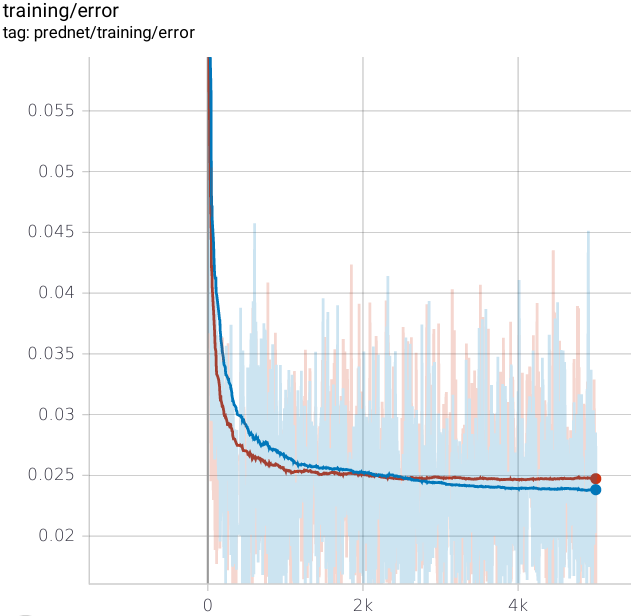
\includegraphics[width=0.55\textwidth]{../Images/prednet_mnist_training.png}
    \centering
    \caption{Training PredNet with ConvLSTM (blue) and PredRNN (red) on MovingMNIST.}
    \label{fig:prednet_mnist_training}
   \end{figure}\noindent
   \begin{figure}[H]
   \centering
   \subfloat[Ground truth]{{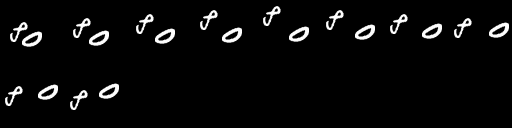
\includegraphics[width=0.6\textwidth]{../Images/prednet_mnist_groundtruth.png} }} 
   \qquad
   \subfloat[ConvLSTM]{{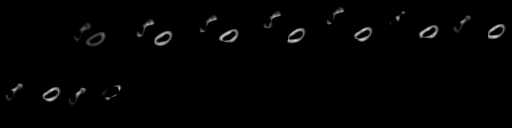
\includegraphics[width=0.6\textwidth]{../Images/prednet_mnist_convlstm_prediction.png} }} 
   \qquad
   \subfloat[PredRNN (vanished)]{{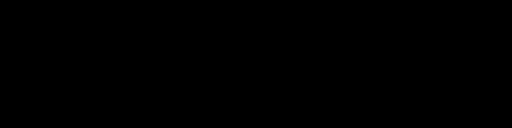
\includegraphics[width=0.6\textwidth]{../Images/prednet_mnist_predrnn_prediction.png} }}
   \caption{Test results for PredNet on MovingMNIST.}
   \label{figure::prednet_mnist_results}
  \end{figure}\noindent
  Here one can see a problem, that was always present during training. The values for MovingMNIST were vanishing very fast, which often resulted in empty images,
  for ConvLSTM and PredRNN. This is due to the fact, that PyTorch is vanishing gradients faster then Keras \cite{chollet2015}, and that Lotter et al. used 
  Matplotlib \cite{Hunter2007}, which is able to catch much smaller values then Tensorboard is (I had to multiply the values with factor ten, to even get some
  output.).
    
  This is one case of using random restarts to have a network which is not vanishing.
   \begin{table}[H]
    \begin{center}
     \begin{tabular}{| l | l | l |}\hline
      \textbf{Model} & \textbf{ConvLSTM} & \textbf{PredRNN} \\\hline
      Autoencoder (Depth $2$) & $0.027$ & $0.028$ \\\hline
      PredNet & $0.035$ & $0.041$ \\\hline
      Spatiotemp & $0.024$ & $0.022$ \\\hline
     \end{tabular}
    \end{center}
    \caption{Mean MSE for MovingMNIST.}
   \end{table}\noindent
   Those values directly show, that the change from ConvLSTM to PredRNN does not make any positive difference for any network performing the tests on MovingMNIST.
   Therefore, as written above, the network using PredRNN only consist of more parameter, so the choice should therefore tend to ConvLSTM, because it has less
   computing time and similar results.
   
  % subsubsection
  \subsubsection{KTH}
   \begin{table}[H]
    \begin{center}
     \begin{tabular}{| l | l | l |}\hline
      \textbf{Model} & \textbf{ConvLSTM} & \textbf{PredRNN} \\\hline
      Autoencoder (Depth $2$) & $542.531$ & $781.760$ \\\hline
      PredNet & $850.325$ & $1.285.730$ \\\hline
      Spatiotemp & $1.007.598$ & $1.421.913$ \\\hline
     \end{tabular}
    \end{center}
    \caption{Number of trainable parameter for KTH.}
   \end{table}\noindent
   \begin{figure}[H]
   \centering
   \subfloat[Ground truth]{{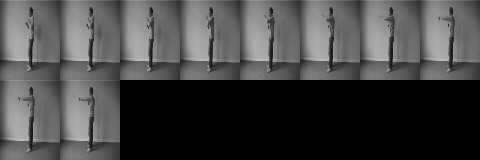
\includegraphics[width=0.6\textwidth]{../Images/prednet_kth_groundtruth.png} }} 
   \qquad
   \subfloat[ConvLSTM]{{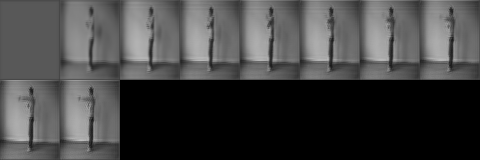
\includegraphics[width=0.6\textwidth]{../Images/prednet_kth_convlstm.png} }} 
   \qquad
   \subfloat[PredRNN]{{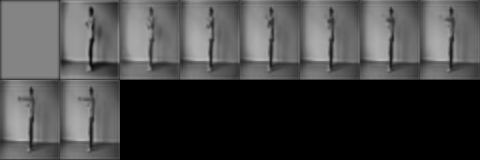
\includegraphics[width=0.6\textwidth]{../Images/prednet_kth_predrnn.png} }}
   \caption{Test results for PredNet on KTH.}
   \label{figure::prednet_kth_results}
  \end{figure}\noindent
   \begin{table}[H]
    \begin{center}
     \begin{tabular}{| l | l | l |}\hline
      \textbf{Model} & \textbf{ConvLSTM} & \textbf{PredRNN} \\\hline
      Autoencoder (Depth $2$) & $1.55e-3$ & $0.05$ (didn't converged) \\\hline
      PredNet & $1.95e-3$ & $1.93e-3$ \\\hline
      Spatiotemp & $3.1e-3$ & $0.025$ (didn't converged) \\\hline
     \end{tabular}
    \end{center}
    \caption{Mean MSE for KTH.}
   \end{table}
  
  % subsubsection
  \subsubsection{Kitti}
   \begin{table}[H]
    \begin{center}
     \begin{tabular}{| l | l | l |}\hline
      \textbf{Model} & \textbf{ConvLSTM} & \textbf{PredRNN} \\\hline
      Autoencoder (Depth $2$) & $542.531$ & $781.760$ \\\hline
      PredNet & $8.222.559$ & $12.430.626$ \\\hline
      Spatiotemp & $1.640.321$ & $2.200.641$ \\\hline
     \end{tabular}
    \end{center}
    \caption{Number of trainable parameter for Kitti.}
   \end{table}\noindent
   \begin{figure}[H]
   \centering
   \subfloat[Ground truth]{{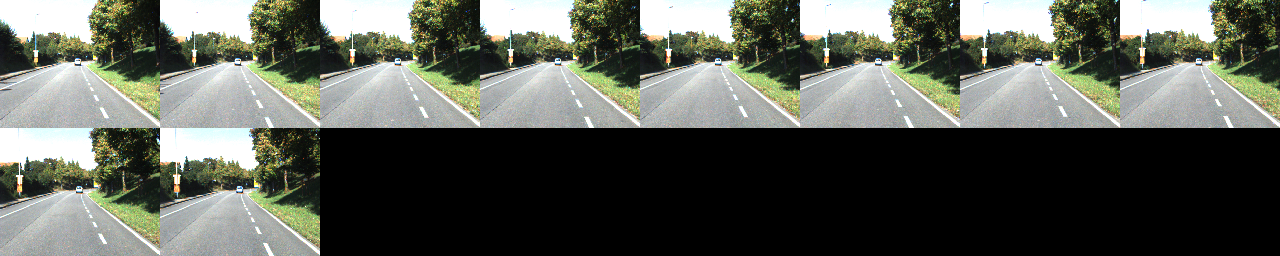
\includegraphics[width=0.7\textwidth]{../Images/prednet_kitti_groundtruth.png} }} 
   \qquad
   \subfloat[ConvLSTM]{{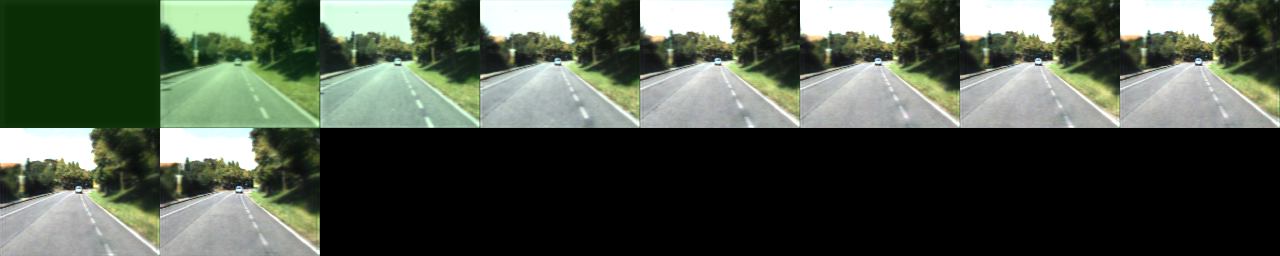
\includegraphics[width=0.7\textwidth]{../Images/prednet_kitti_convlstm.png} }} 
   \qquad
   \subfloat[PredRNN]{{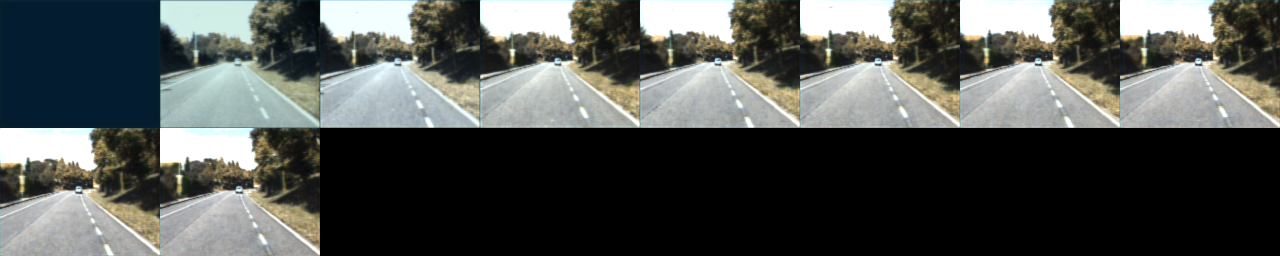
\includegraphics[width=0.7\textwidth]{../Images/prednet_kitti_predrnn.png} }}
   \caption{Test results for PredNet on Kitti.}
   \label{figure::prednet_kth_results}
  \end{figure}\noindent
   \begin{table}[H]
    \begin{center}
     \begin{tabular}{| l | l | l |}\hline
      \textbf{Model} & \textbf{ConvLSTM} & \textbf{PredRNN} \\\hline
      Autoencoder (Depth $2$) & $0.02$ & $0.013$ \\\hline
      PredNet & $0.019$ & $0.02$ \\\hline
      Spatiotemp & $0.018$ & $0.017$ \\\hline
     \end{tabular}
    \end{center}
    \caption{Mean MSE for Kitti.}
   \end{table}